\documentclass[a4paper,titlepage]{report}

\usepackage{geometry}
\usepackage{graphicx}
\usepackage{amssymb}

\geometry{
  includeheadfoot,
  margin=2.54cm
}

\begin{document}

\begin{titlepage}

\begin{center}
 
\Large\textbf{Department of Physics and Astronomy\\
University of Heidelberg}

%change back when submitting
%\vspace{18cm}

\vspace{16cm}

\normalsize
Bachelor Thesis in Physics\\
submitted by\\
\vspace{0.5cm}
\Large\textbf{Maximilian Argus}\\
\normalsize
\vspace{0.5cm}

born in Hamburg, Germany\\
\vspace{0.5cm}
\Large\textbf{1990}
\normalsize

\newpage




\Large\textbf{Electric Field Optimization of a Rydberg Atom Experiment}

\vspace{18cm}

\normalsize
This Bachelor Thesis has been carried out by Maximilian Argus at the\\
Physikalisches Institute in Heidelberg\\
under the supervision of\\
Prof. Dr. Matthias Weidem\"uller

\vfill
\end{center}

\end{titlepage}


\begin{abstract}
Modern experiments with ultracold Rydberg atoms with application to many body physics and quantum information science, demand a  high level of experimental sophistication to precisely control experimental parameters like external electric fields, as Rydberg atoms are very  polarizable. In the experiment this is achieved by (a structure hosting) >10 individually controllable electrodes. However, the task of finding the optimal control voltages for these is complicated by incomplete knowledge of the charge distributions, including possible patch fields (making it particularly time consuming). To overcome this challenge we have applied evolutionary algorithms, a group of powerful search heuristics, to optimize the overall performance of our experiment. With particular focus on electric field control we asses the performance of several algorithms, on competing requirements of noise robustness and fast convergence, in solving two problems: cancellation of electric fields and and optimum guiding of field ionized Rydberg atoms to a MCP detector. Additionally Foreseeable applications to controlling quantum state evolution and engineering strongly correlated many body systems of interacting Rydberg atoms will be considered. 

\end{abstract}



\section*{Introduction}
Introduction introduction introduction

\tableofcontents

\chapter{Concept}

The aim of this thesis is the application of optimization methods to a Rydberg atom experiment. In the course of making one measurement several steps have to be completed sequentially. These start with collecting Rubidium atoms into a MOT, pre-cooling then and then loading them into a diplote trap where they are exited into Rydberg atoms. After this has been done the atoms can be imaged by a camera system. These steps form a cycle that is repeated every few seconds with variation of parameters in order to make measurements of the change in beahaviour of the Rydberga atoms dependends on the varied parameters. While many properties of the experimental setup are physically fixed, such as the position of the lasers, a relativley large number (77) that can be controlled by the software controlling the experiment, such as the timing of activating these lasers. The aim of this project is to add information feedback to this cycle, so that the experiment can choose new experimental parameters based the results of previous evaluations. The scematic for this is shown in figure 1.1

\begin{figure}[htb]
\centering
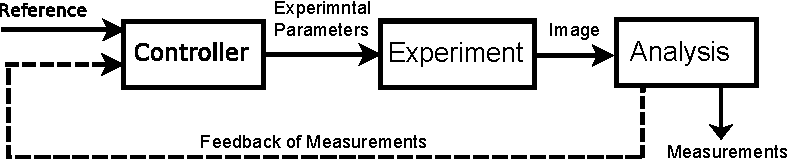
\includegraphics{Images/Feedback.pdf}
\caption{Information Feedback}
\label{fig: Information Feedback}
\end{figure}


Due to the discrete nature of experimental cycle evaluations and the large number of paramters as well as considerable measurement noise an opimization approach was choosen that generates and evaluates new experimental parameters. Using one can define the goal of the optimization as a function of several of the measurement results calculated by the analysis step.

Of particular interest is the control of experimental electrodes sourrounding the Rydberg atoms. One of the experimental goal is creating minimal electric fields as the predictions that are made assume a field-free environment. Additionaly it is important to generate a homogeneous filed as this prevents position dependent energies. When working with Rydberg atoms one mostly want to increase the principle quantum number $n$ in order to scale with it the physical effects one is trying to measure, however the polarizability of Rydberga atoms scales with $n^7$ requiring fine control over the electric field if one wants to work with larger Rydberg atoms.



\chapter{Theoretical Background}

\chapter{Optimization}

\section{Mathematical Formulation}
A $n$ dimensional real value optimization problem can be stated in the form
\[ min f(\mathbf{x})  \]
for
\[ f: S \rightarrow  \mathbb{R} \]
where
\[ \mathbf{x} \in S  \subseteq \mathbb{R}^n \]

\noindent
A point $\mathbf{x}^* \in D$ is a global minimum if  $ f(\mathbf{x}^*) \leq f(\mathbf{x}^*)  \forall  \mathbf{x} \in S$

\noindent
A point $\mathbf{x}^* \in D$ is a local minimum if  in the surrounding  $ U \subseteq S$ of  $\mathbf{x}^*$ it holds that $f(\mathbf{x}^*)  \leq f(\mathbf{x})  \forall  \mathbf{x} \in U$


\section{Background: Why look at multiple algorithms?}
There are a large number of optimization algorithms that have been developed in order to solve different problems. The key to applying optimization algorithms then is to find one suitable to solving kind of problems one is working with. Abstractley this is the converse to the No Free Lunch Theorem which states that the average performance of an optimizationa algorithms, when applied to the set of all optimization problems,  does not outperforom any other optimization algorithm or random walk. An algorithm is thus only, compartivley, suitable if it is able to utilize some form of problem specific information coupling the choice of algorithm to the problem at hand.

Due to the kind of problems to which optimization is to be applied to only the subset of Monte Carlo probablistic global optimization algorithms will be considered. These algorithms sacrifice both evaluating the entire search space and the necessity of evaluating the function exactly in favour of a shorter runtime. In these algorithms the choice of which candidates to evaluate is made by a heuristic which makes an induction based on previous evaluations. It is in this heuristic that is represents the problem specific information of the optimization algorithm.


\section{Evolutionary Algorithms}

Evolutionary Computation repersents a subset of heuristic based approaches in which a set of possible solution candidates is maintained which the algorithm tries to refine over a number of generations. In the following sections we will introduce the differnt categories of algorithms used as well as the specific implementations of algorithms from these categories.

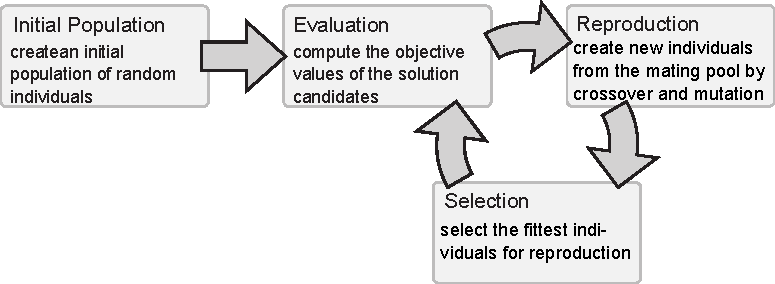
\includegraphics{Images/evolution_v2.pdf}

\subsection{Population Size}
\subsection{Exploration//Exploitation}


\section{Swarm Intelligence}

\section{Evolutionary Computation}

\chapter{Implementation}

The application of optimization directly to the Rydber experiment posed a number of difficulties in that the parameters for optimization on the physical experiment were very different from those which numerical optimization is usually applied to, while it is possible to evaluate a numerical function or simulation very quickly and or in parrael there was a strong constraint on the number of evaluations of solution candidates. In order to still be able to achieve convergence of the optimization algorithm this required a reduced dimensionality of the problem that we were attempting to solve. In addition to this physical measurements are also affected by noise. These conditions were used to choose an appropriate algorithm that could be applied the the experiment.

\section{Test Function}
In order to evaluate the different algorithms that are avaliable a mathematical test problem was formulated. This problem could then be evaluated by computer allowing for the large number of evaluations needed to compare the algorithm with different paramaters and compare the results to other algorithms. In order to make this comparison meaningfull one needs to choose a test problem that matches the actual experiment as closley as possible, to do this a $n$ dimensional Gaussian was choosen.

To further increase similarity with the experiment three sources of noise were added: measurement noise affecting the amplitude of the function($\sigma_a$), backgorund noise added to the fucntion($\sigma_b$) and noise in the parameters that were passed to the function$\sigma_p$. 

\[g(x_i,\sigma) = e^{\frac{(x_i^*-x_i)^2}{2\sigma}}\]
\[G(\mathbf{x},\sigma) = \prod_{i=1}^n g(x_i, \sigma)\]
\[f(\mathbf{x}) =  \mathcal{N}(1,\sigma_a) * \prod_{i=1}^n g(\mathcal{N}(x_i,\sigma_p), \sigma) + \mathcal{N}(0,\sigma_b) \]

As we know only little about the problem landscape of the actual experimental paramters that we are going to optimize this test problem represents a best guess, strictly speaking we cannot induce the suitability to application in the experiment of the algorithm choosen according this test function, however it will be attempted as notheless as it is the best starting point avaliable.


\section{Comparison of Algorithms}




\newpage
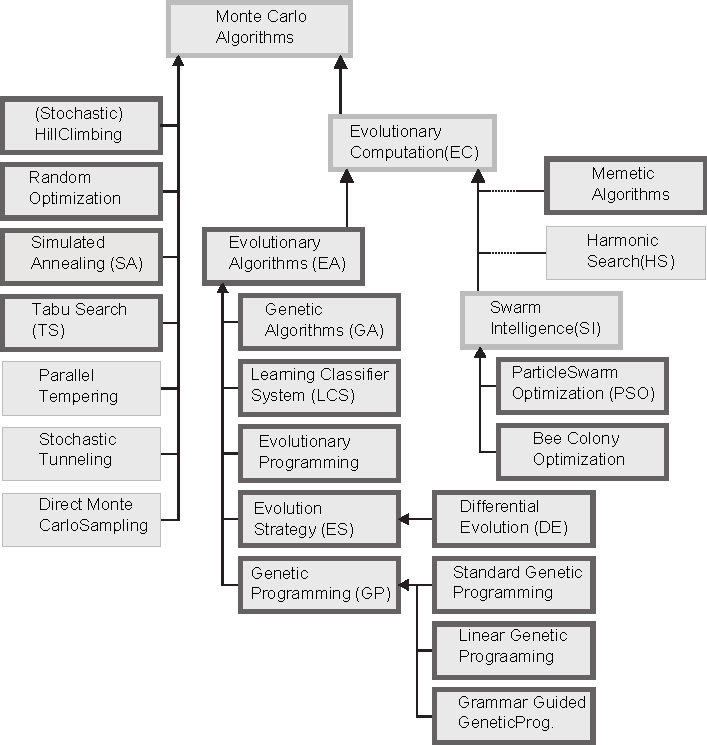
\includegraphics{Images/taxonomy_v2.pdf}

\section{Appendix}


\end{document}